%-----------------------------------------------------------------------------
%
%               Template for sigplanconf LaTeX Class
%
% Name:         sigplanconf-template.tex
%
% Purpose:      A template for sigplanconf.cls, which is a LaTeX 2e class
%               file for SIGPLAN conference proceedings.
%
% Author:       Paul C. Anagnostopoulos
%               Windfall Software
%               978 371-2316
%               paul@windfall.com
%
% Created:      15 February 2005
%
%-----------------------------------------------------------------------------


\documentclass[preprint]{sigplanconf}

% The following \documentclass options may be useful:
%
% 10pt          To set in 10-point type instead of 9-point.
% 11pt          To set in 11-point type instead of 9-point.
% authoryear    To obtain author/year citation style instead of numeric.

\usepackage{amsmath}
\usepackage{syntax}
\usepackage{url}
\usepackage{graphicx}
\usepackage{qtree}

\begin{document}

\conferenceinfo{PPOPP '12}{date, City.} 
\copyrightyear{2011} 
\copyrightdata{[to be supplied]} 

\titlebanner{DRAFT}        % These are ignored unless
\preprintfooter{draft version}   % 'preprint' option specified.

\title{Towards Parallel and Distributed Programming using Bottom-Up Logic Programming}

\authorinfo{Flavio Cruz \and Ricardo Rocha}
           {CRACS \& INESC-Porto LA, Faculty of Sciences, University of Porto\\
                  Rua do Campo Alegre, 1021/1055, 4169-007 Porto, Portugal}
           {\{flavioc,ricroc\}@dcc.fc.up.pt}
\authorinfo{Michael Ashley-Rollman \and Seth Copen Goldstein}
           {Carnegie Mellon University, Pittsburgh, PA 15213}
           {\{mpa,seth\}@cs.cmu.edu}

\maketitle

\begin{abstract}
In the last few years there as been a steady increase of processing power.
Multicore processors are now increasingly prevalent and networks of commodity computers
present an opportunity to solve bigger problems. Programming in these kinds of
systems is not as simple as it should be since optimizing programs to run on
different types of distributed systems is notoriously hard.
We propose a logic programming language based on Datalog
that is suitable for developing general purpose programs for
both parallel and distributed systems. The language uses the notion of
link restricted rules for parallelizing computation
and \emph{action facts} for doing input/output.
We developed a compiler and a runtime system with several execution strategies,
from multithreaded execution to distributed execution using MPI. We also
developed several techniques based on XY-stratification to reduce memory usage.
Finally, we present several application cases, from graph problems to machine learning
algorithms.
\end{abstract}

\category{CR-number}{subcategory}{third-level}

\terms

\keywords

\section{Introduction}

The last decade has seen a priority shift for processor companies. If clock frequency
was once the main metric for performance, today computing power is measured in number of
cores in a single chip.
For software developers and computer scientists, once focused in developing sequential programs,
newer hardware usually meant faster programs without any change to the source code. Today,
the free lunch is over. Multicore processors are now forcing the development of
new software methodologies that take advantage of increasing processing power.
However, parallel programming is difficult, usually because programs are written
in imperative stateful programming languages that make use of relatively low level synchronization
primitives such as locks, mutexes and barriers. This tends to make the task of managing multithreaded
execution quite intricate and error-prone, resulting in race hazards and deadlocks.
In the future, \emph{many-core} processors will make this task even more daunting.

On the other hand, advances in network speed and bandwidth are making distributed computing
more appealing. For instance, \emph{cloud computing} is a new emerging paradigm that wants
to make every computer connected to the Internet connected to the same pool of computing power,
where data can be retrieved and computation can be done. For high performance computing, the
\emph{computer cluster} is a well established paradigm that uses fast local area networks to
improve performance and solve problems that would take a long time with a single computer.

Developments in parallel and distributed programming have originated several programming models.
At the end of the spectrum are lower-level programming abstractions such as
\emph{message passing} (e.g., MPI~\cite{gabriel04-open-mpi}) and \emph{shared memory}
(e.g., Pthreads and OpenMP~\cite{Chapman-2007-UOP-1370966}).
While such abstractions are very expressive and enable the programmer to write very performant code,
they tend to be very hard to use and debug, due to synchronization problems, making it difficult to
prove the program's correctness.

An approach that attempts to address the correctness challenges, is to use declarative languages
such as \emph{logic programming languages} or \emph{functional programming languages}. In logic languages such
as Prolog, researchers took advantage of the non-determinism of proof-search to evaluate subgoals
in parallel with models such as \emph{or-parallelism}~\cite{ali-86} and \emph{and-parallelism}~\cite{Shen-92}. In functional languages, the stateless nature of computation
allows multiple expressions to evaluate safely in parallel. This has been explored in several languages
such as NESL~\cite{Blelloch:1996:PPA:227234.227246} and Id~\cite{Nikhil93anoverview}.

Recently, there has been an increasing interest in declarative and data-centric languages.
MapReduce~\cite{Dean:2008:MSD:1327452.1327492}, for instance, is a popular data-centric programming
model that is optimized for large clusters. The scheduling and data sharing model is very simple:
in the \emph{map phase}, data in each node is transformed and in the \emph{reduce phase}, nodes
communicate to compute the final result.

A declarative approach that is becoming popular is Datalog~\cite{Ullman:1990:PDK:533142}, a
bottom-up logic programming language.
Traditionally used in deductive databases, Datalog is being increasingly used in different fields
such as: distributed networking~\cite{Loo-condie-garofalakis-p2}, sensor nets~\cite{Chu:2007:DID:1322263.1322281} and cloud computing~\cite{alvaro:boom}.

In the context of the Claytronics project~\cite{goldstein-computer05}, a massive distributed system
we've been using a Datalog variant called Meld~\cite{ashley-rollman-iclp09, ashley-rollman-derosa-iros07wksp}.
Meld is specially suited for writing programs for distributed systems where the network
topology can change dynamically. Such systems are called \emph{ensembles} and they include
programmable sensor networks and modular robotic systems.

We now have been adapting Meld to implement general parallel algorithms in multicore machines
and clusters. We extended the language with lists and reduced the need to do deletion.
We are using the concept of \emph{action facts} to model output.

We have implement a new compiler and a virtual machine that is able to execute on multicore machines
and distributed networks. For multicore machines we have implemented different scheduling schemes,
including static division of work and work stealing.
For distributed networks and clusters we are using MPI with a static division of work.
Finally, the runtime system is able to take advantage of multicores when doing distributed computation.

The rest of the paper is organized as follows. In the next section we describe the Meld language
and the modifications we made to make it more suitable for parallel programming. Next, we present
how the runtime system distributes the computation across processors and machines and the different
scheduling schemes. In Section~\ref{sec:evaluation} we evaluate the language modifications with
several applications from graph theory and machine learning. Finally, we end the paper outlining
some conclusions and further work.

\section{The Meld Language}

Meld is a bottom-up logic programming language based on Datalog. Like Datalog, it
consists of a database of \emph{facts} and a set of \emph{production rules} for generating new facts.
Each fact is an association between a \emph{predicate} and a tuple of values. A predicate can be seen
as a relation or table in which the tuples are its elements. Production rules have the form
$\mathtt{p :- q_1, q_2, ..., q_n.}$, meaning that "if $\mathtt{q_1}$ and $\mathtt{q_2}$ and ... and
$\mathtt{q_n}$ are true then $\mathtt{p}$ is true".

\subsection{Evaluation}

When a Meld program starts executing, the set of initial axioms in the form $\mathtt{p.}$ are
instantiated and added to the database. With these new facts, rules are then fired and new
facts are generated and added to the database, until a \emph{quiescent} state is reached, where
no more facts can be generated. In Meld, we can also have \emph{action facts},
which are syntactically similar to regular facts but cause some side effect. In the context of
modular robotics, action facts activate the robot's actuators in order to produce movement
or control devices. For parallel programming we use the concept of action facts for writing
results to files. Note that action facts are not added to the database.

\subsection{Rules}

A Meld program contains a set of rules. A rule has two main components: the \emph{head},
which indicates the facts to be generated; and the \emph{body}, which contains the pre-requisites
to generate the head facts. The body may contain the following as pre-requisites: \emph{subgoals},
expression constraints or/and variable assignments. The head can only contain subgoals.
Variables are limited to the scope of the rule and must be defined in the body facts or through
the body variable assignments. Variables that only appear on the head are forbidden, since each
instantiated fact must have only \emph{ground facts} and thus all arguments must be instantiated.

Whenever all body pre-requisites are satisfied, the head subgoals are instantiated as
facts and then they are added to the program database (except when action facts are derived).
To satisfy all pre-requisites, the body
subgoals must be matched against the program database. Both constraints and subgoals
match when consistent substitution is found for the body's variables such that one or
more facts in the database are matched. Constraint expressions are boolean expressions that
use variables from subgoals (and thus database facts) and from variable assignments. Allowed
expressions in constraints include arithmetic, logical and set-based operations.

Each predicate used in the program must be explicitly typed. Each field is either of a basic
type or a structured type. Basic types include the integer type, floating point numbers and
the \emph{node address} (see \ref{sec:localization}).
A structured type includes lists of basic types. Syntax-wise, lists have a Prolog-like syntax.

\begin{grammar}
<rule> ::= <ident> ‘=’ <expr>
\alt ‘for’ <ident> ‘=’ <expr> ‘to’ <expr> ‘do’ <statement>
\alt ‘{’ <stat-list> ‘}’
\alt <empty>
<stat-list> ::= <statement> ‘;’ <stat-list> | <statement>
\end{grammar}

\subsection{Aggregates}

In contrast to Datalog, Meld does not have negation, but has \emph{set aggregates}
\footnote{It has been shown in~\cite{zaniolo-arni-ong-dood93} that set aggregates can be
implemented using negation, however we implement aggregates directly, without using source
code transformation.}. The purpose of an aggregate is to define a type of predicate that combines
the facts of that predicate into a single fact. The definition of an aggregate includes the
field of the predicate and the type of operation to be done on the collection of facts.

Consider a predicate $\mathtt{p(f_1, ..., f_{m-1}, agg\ f_{m}, f_{m+1}, ..., f{m+n})}$,
where $f_m$ is the aggregate field associated with the operation $\mathtt{agg}$. For each
combination of values $\mathtt{f_1, ..., f_{m-1}}$ there will be a set of facts matching
the same combination. To calculate the aggregated fact of each collection, we take all
the $\mathtt{f_{m}}$ fields and apply the $\mathtt{agg}$ operation. The fields between
$\mathtt{f_{m+1}}$ and $\mathtt{f_{m+n}}$ for the aggregated fact are chosen depending
on the operation.

Meld allows several aggregate operations, namely: \texttt{max}, to compute the maximum value;
\texttt{min}, to compute the minimum value; \texttt{sum}, to sum all the values of the corresponding
fields; and \texttt{first}, to select the first fact field.

\subsection{Localization}\label{sec:localization}

Another difference between Meld and Datalog, is that in the former, the first field
of each predicate indicates must have the type node address.
In rules, the first argument of each subgoal is called the \emph{home variable} and
refers to the node where the fact will be stored, so that each node has its own database.

This convention originated in the context of declarative networking~\cite{Loo-condie-garofalakis-p2},
in the P2 system. For modular robotics, this makes it trivial to
distribute data across the ensemble. In the context of this paper, each fact is a
\emph{structural fact} and can be seen as part of the data structure representing a node in the graph.
Moreover, when each fact is associated with a certain node, it helps us distribute
and parallelize computation and also improve data locality (see~\ref{sec:topology}).

While each fact must be associated with some node, a rule may contain subgoals that refer to
different nodes. In order to simplify rule activation, the rules are transformed so that
each subgoal refers to the same node. The process of \emph{localization} is fundamental
in the distribution of computation.

Before localization, each rule can be either a \emph{local rule} or a \emph{link-restricted rule}.
A local rule does not need to be transformed since only facts from a single node are needed.
A link-restricted rule is a rule where subgoals may refer to different nodes. This type of rule
must be transformed so that the right subparts of the rule are matched
on the right nodes (by matching the facts of that node only)
and the instantiation of the head subgoals into facts is done on the subgoal the head subgoals
refer to. To accomplish this, the nodes involved in the computation of the rule must communicate
between each other so that the rule is fired when everything has been known to match.
For this, we introduce a special class of facts called the \emph{link facts}. These facts
represent the edges in the graph and force the nodes to do direct communication with
only their direct neighbors.

For an example, consider the following block of Meld code, where a rule refers to three different
nodes, \texttt{A}, \texttt{B} and \texttt{C}.

\begin{verbatim}
fact2(A, 2) :-
   fact1(A, A1), A1 > B1,
   edge(A, B), fact1(B, B1), B1 > C1,
   edge(A, D), fact1(D, D1),
   edge(B, C), fact1(C, C1).
\end{verbatim}

To localize this rule, we first build a tree representing the connection paths between nodes by
picking an arbitrary root node, in this case, the node \texttt{A}, and then by adding
edges using link facts. The resulting tree is represented in Fig.~\ref{fig:loctree}.
Note how the constraints were placed in the first node where all the variables used in the constraint
were available. This optimization aims to reduce communication by testing constraints as soon as
possible.

\qtreecenterfalse
\begin{figure}[ht!]
\scalebox{0.75}{
\Tree [.{\bf A} [.{\bf B} [.{\bf C} {\tt fact1(C, C1)} ] {\tt{fact1(B, B1),}\\$\mathtt{B1 > C1}$} ] [.{\bf D} {\tt fact(D, D1)} ] {\tt fact1(A, A1),\\ {\tt A1 $>$ B1}} ]
}
\caption{Localization tree}
\label{fig:loctree}
\end{figure}

Once connection paths are known, localization transforms the original rule into several
\emph{send rules}, that are characterized by having the same node in the body and a different
node in the head. Once a send rule body matches,
all the subgoals in the head are instantiated and then sent to the corresponding node,
where the matching of the original rule can continue, until the complete rule matches.
The following code shows the final result.

\begin{verbatim}
__edge(X, Y) :- edge(Y, X).

fact2(A, 2) :-
   fact1(A, A1), A1 > B1,
   __remote1(A, B1), __remote3(A).
   
__remote1(A, B1) :-
   __edge(B, A), fact1(B, B1), B1 > C1,
   __remote2(B, C1).
__remote2(B, C1) :-
   __edge(C, B), fact1(C, C1).
__remote3(A) :-
   __edge(D, A), fact1(D, D1).
\end{verbatim}

\subsection{Pipelined Evaluation}

Evaluation of Datalog programs (including programs with recursive rules) can be done using
several techniques, one of the most well-known being the \emph{semi-naive fixpoint}
evaluation~\cite{Balbin1987259, Bancilhon:1986:NER:8789.8804}. However, these techniques
are more appropriate for a centralized evaluation and are expensive in a distributed environment,
because they require global synchronization. To this end, we use the \emph{pipelined semi-naive}
evaluation from P2~\cite{Loo-condie-garofalakis-p2}, which relaxes the semi-naive fixpoint
by making the concept of iteration local to a node.

Whenever a new fact is generated by the node or sent by a neighbor node, the fact is added to local
queue which contains all new facts. As execution proceeds, a fact pulled out of the queue. Then,
all rules that use the fact in their body are selected as candidate rules. For each candidate, the
rest of its rule body is matched against the facts in the database. If the rule is proved, the subgoals
in the head of the rule are instantiated and added to the local queue as new facts.

\subsection{Example: Shortest-Path}

For an example, consider the program in Fig.~\ref{fig:shortestpath} that computes the
shortest distance and the corresponding path between any node to node 4.
Each edge in the graph is represented
by the \texttt{edge} relation in \texttt{r4}, and includes the source node, the destination node and
the distance of the connection. Note how node addresses are prepended with the symbol @.

\begin{figure}
\begin{verbatim}
type end(node).
type route edge(node, node, int).
type path(node, min int, list node).

r1: path(A, W, [A, B]) :-
      edge(A, B, W),
      end(B).

r2: path(A, D + W, [A | P]) :-
      edge(A, B, W),
      path(B, D, P).
  
r3: write_int(A, W), write_list(A, P) :-
      terminated(A),
      path(A, W, P).
  
r4: edge(@0, @1, 1). edge(@1, @2, 1).
    edge(@2, @3, 3). edge(@0, @2, 4).
    edge(@2, @0, 2). edge(@1, @4, 2).

r5: end(@4).
\end{verbatim}
\caption{Shortest Path in Meld}
\label{fig:shortestpath}
\end{figure}

The \texttt{path} predicate is a transitive closure
subject to an aggregated field, which forces the selection
of the fact with the least distance. In \texttt{r1}, we define the path
for each neighbor node of node 4, by declaring that a node \texttt{A} has an edge to node \texttt{B}
and node \texttt{B} is the selected final node.
In \texttt{r2} we complete the transitive closure, declaring that the shortest path between \texttt{A}
and a node \texttt{B} is the sum of the distance between \texttt{A} and \texttt{B} and the
shortest distance between \texttt{B} and node 4.

\begin{figure}[ht]
  \centering
    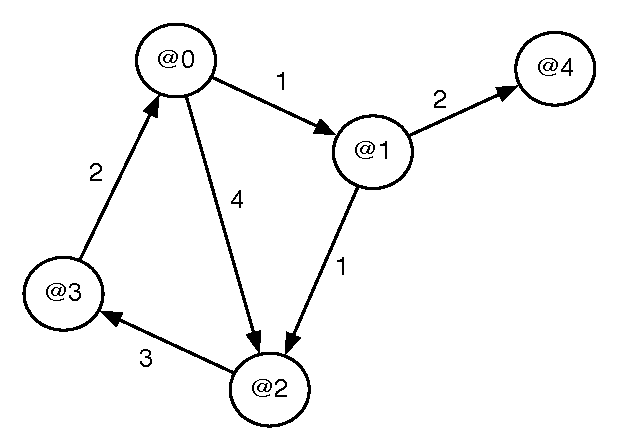
\includegraphics[width=0.28\textwidth]{figures/shortestpathgraph.pdf}
  \caption{Shortest path graph.}
  \label{fig:shortestpathfig}
\end{figure}

Using the localization method, we know that node 4 will send a fact representing
a match of rule r1 to its neighbors, in this case, node 1. Node 1 then instantiates a new
path fact \texttt{path(@1,~2,~[@1, @4])}. At this moment, node 1 could generate the aggregated
\texttt{path} fact representing the least path to node 4 or could wait until all the \texttt{path}
are generated.

In a distributed setting, it is difficult to assess if all facts of an
aggregate collection are already on the database (we present techniques to avoid this in XXX).
However, we use a technique borrowed from P2 called \emph{deletion} that allows Meld
to retract facts derived from invalid facts such as aggregates based on partial information
or changes in the environment (in the case of modular robotics). Deletion
is presented in detail in the next section.

In this case of this graph (Fig.~\ref{fig:shortestpathfig}), node 1 can generate the least path
safely and send it to node 0. Node 0 receives this fact and generates a new aggregate: \texttt{path(@0,3,[@0,@1,@4])}. Node 0 then sends a new fact to node 3, node 3 generates a
new aggregate and generates a new fact that is sent to node 2. Node 2 then generates its
least path aggregate: \texttt{path(@2,8,[@2,@3,@0,@1,@4])} and fires rule r2 for neighbors
node 0 and node 1. However these new paths are not minimal and thus nothing is generated,
resulting in a fixpoint in the graph. If, however, a better path was found, the everything
derived from the old path would have to be deleted and the new path added to the database.

\subsection{Deletion}

Deletion is mechanism that allows Meld to delete all facts derived from invalid facts such
as aggregates based on partial (and incomplete) information. In the context of modular robotics,
deletion is used to delete everything derived from old world information and thus keep the database
of facts consistent to the robot's environment.

Deletion works by considering a deleted fact and matching the rules in exactly the same way as
derivations are done to determine which facts depend on the deleted one.


\subsection{Aggregates and Recursive Rules}

\cite{zaniolo-arni-ong-dood93}

\subsection{XY Stratification and Remote Rules}

\subsubsection{Aggregate modifiers}

\section{Parallel Execution}

\subsection{Topology Ordering}\label{sec:topology}

\subsection{Selective Localization}

\subsection{Scheduling}

\subsubsection{Multithreading}
\subsubsection{Distributed}
\subsubsection{Mixed Mode}

\section{Evaluation}\label{sec:evaluation}

In this section we present several programs written Meld that show possible
uses of the language.

\subsection{All-Pairs Shortest Path}

\subsection{PageRank}

\subsection{Belief Propagation}

\subsection{Neural Networks}

\section{Conclusions and Further Work}

bla bla linear logic state bla bla splash bp

\acks

% We recommend abbrvnat bibliography style.

\bibliographystyle{abbrvnat}

% The bibliography should be embedded for final submission.

\bibliography{refs}

\end{document}
